\chapter{Quid du projet SocFace?}
L’objectif de SocFace est très simple : numérisation des listes de recensements français de 1836 à 1936 et extraction des informations pour créer une base de données. Ce qui est moins évident, c’est d’une part la mise en œuvre et d’autre part, la gestion des résultats escomptés. Ce sont de fait les chiffres qui impressionnent le plus et qui font toute la singularité de SocFace. On se demandera d’ailleurs si on peut parler de Big Data pour les données du projet. 



    \section{Objectifs du projet}

Les listes des \gls{LNR}\footnote{Voir Glossaire} sont conservées en grande majorité dans les Archives Départementales et les Archives Municipales des grandes villes. L’un des objectifs du projet est donc de favoriser la collaboration entre les services d’archives et les acteurs du projet. La très grande majorité de ces archives avaient déjà numérisé les listes de recensement.\\
Le principe de dénombrement via le recensement commence en 1836. Il est à noter que quelques expériences avaient été tentées auparavant : des dénombrements fiscaux, des enquêtes par les intendants, sous Louis XIV et Louis XV. Mais ces listes sont des initiatives locales et n'ont pas le caractère imposé, sériel et national des listes de recensement qui commencent en 1836. Ces listes se font par commune et dénombrent individuellement la population. Elles sont classées par rues, puis chaque habitant est dénombré par famille : le chef de famille en tête, puis son épouse, ses enfants, et les autres membres du ménages, qu’ils soient membres de la famille
ou non (les personnes employées par le ménage, en particulier les domestiques, ou simplement logés par lui). Différentes informations sont fournies sur chaque individu, variable au cours du temps. Mais on retrouve de façon à peu près constante : le nom, prénom, âge (ou année de naissance), position dans la famille, profession et nationalité (depuis 1851).\\
    
    \begin{figure}[H]
        \centering
        \includegraphics[width=0.8\linewidth]{Figures/Partie 1/Fig.1.1 - LNR Eygalières.png}
        \caption[Extrait du recensement des Bouches du Rhône - de 1861 pour le village d'Eygalières]{Extrait du recensement des Bouches du Rhône de 1861 pour le village d'Eygalières}
        \label{fig:Fig1.1}
    \end{figure}

L’objectif principal est de produire une base de données qui reprend toutes ces informations. Les images sont classées par service fournisseur d'archives, en général au niveau départemental, puis par année et enfin par commune. La base de données permet donc de naviguer dans toutes ces informations et retrouver le nom d’un habitant en particulier, ou à l’inverse le nom de la commune et même de la rue dans laquelle habitait une personne. Ce type de recherche existe déjà, développé par la communauté des généalogistes. Les bases de données de ces communautés sont généralement basées sur des indexations d’état civil fait par des passionnés, "à la main". On y trouve des associations départementales, comme les bases RECIF pour le Finistère ou bien des logiciels à visée nationale comme Généanet\footnote{\href{https://www.geneanet.org/}{https://www.geneanet.org/}} ou MyHeritage\footnote{\href{https://www.myheritage.fr/}{https://www.myheritage.fr/}} (payants) ou ELIE\footnote{\href{https://www.mcs-gen.com/}{https://www.mcs-gen.com/}} (gratuit).\\

En France, d'autres projets ont adopté une démarche similaire.  Le CNRS, en partenariat avec le laboratoire informatique \gls{LITIS} porte le projet POPP, dont le périmètre est recentré sur Paris durant l’entre-deux guerres (1926-1946). Ce projet s’est doublé du projet EXO-POPP, qui concerne les actes de mariages de Paris et sa banlieue sur la même période. Un immense projet a également été mené par le Ministère de la Défense : \textit{Mémoire des hommes}\footnote{\href{Mémoire des hommes}{https://www.memoiredeshommes.sga.defense.gouv.fr/}}. Commencé en 2003 et refondu en 2013, ce site internet permet de rechercher les soldats ayant participé à la plupart des guerres françaises du XXe siècle, les morts pour la France, les sépultures... Le site s'est enrichi de la numérisation des collections du ministères, créant une base de données de 2,7 millions de noms et 5 millions d'images. 
A l'étranger, on peut mentionner le projet québécois BALSAC. Depuis 1972, l’UQAC numérise les \gls{AEC} et relie les informations pour permettre de retracer les familles et les lignées généalogiques. Des millions de documents ont été traités depuis plus de 50 ans, et la base de données est accessible aux chercheurs. Ce projet est d'une ampleur considérable mais n'utilise pas la même technologie que SocFace, qui cherche à numériser dans un temps beaucoup plus court un nombre tout aussi considérable d'images. Il y a également IPUMS\footnote{\href{IPUMS}{https://www.ipums.org/mission-purpose}}, un ambitieux projet américain de l'université du Minnesota qui centralise et rend accessible des microdonnées provenant de recensements et d'enquêtes démographiques du monde entier. L'organisme travaille avec 105 agences nationales de statistiques, 9 services d'archives et des sites de généalogies et gèrent des milliards d'enregistrements. La différence avec SocFace est que beaucoup de ces données sont déjà numériques, et la lecture de recensement "anciens", beaucoup plus réduite. Mais IPUMS reste une référence pour SocFace.\\
Ces projets sont donc semblables mais n'utilisent pas nécessairement les lecture optique des \gls{LNR} et leurs sources sont différentes. SocFace est le premier projet à numériser - en France - l'ensemble des listes de recensements. Mais ils ont en commun leur taille, puisque chacun produit un nombre de données important. 

    \section{Les chiffres}

La collecte des fichiers numérisés des listes du recensement se fait auprès de l’ensemble des départements français. En accord avec le \gls{SIAF}, les services d’archives ont le choix de participer au projet ou non. Dans l’ensemble, la collecte s’est révélée être un succès : sur les 108 services d'archives contactés (départementales et municipales), 98 ont donnés leur accord \footnote{Voir Annexe F}.  

      \begin{figure}[H]
        \centering
        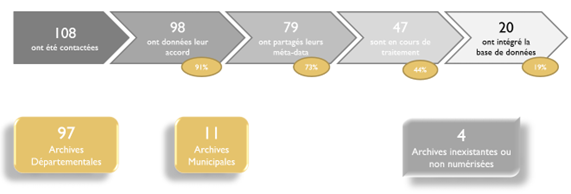
\includegraphics[width=0.9\linewidth]{Figures/Partie 1/Fig.1.2 - Participation des services d'archives.png}
        \caption[Participation des services d'archives]{Participation des services d'archives}
        \label{fig:Fig1.2}
    \end{figure}

Parmi les 20 services ayant décliné, les raisons sont multiples : pour certains, les fichiers n'ont pas encore été numérisés, ou pas en totalit, pour d'autres, les archives ont disparues. Enfin, certains n'ont pas encore répondu ou ont refusé de participer (seulement un service jusqu'ici).

SocFace demande aux services d’archives de verser les images ainsi qu’un fichier comprenant les métadonnées qui leur sont associées. Sur les 98 services d’archives ayant accepté le projet, 79 ont déjà envoyé ces fichiers, parfois avec des informations manquantes. Il faut également noter que certaines années ou communes sont manquantes, pour diverses raisons. A ce jour, la collecte d’image se chiffre à 10 557 555. La projection finale est à 15 millions d’images, ce qui représente un stockage de 3 Téra octets. Voici un tableau comparatif\footnote{Ressources utilisées pour la création du tableau : \\ 
\href{https://ischoolonline.berkeley.edu/blog/big-data-infographic/}{https://ischoolonline.berkeley.edu/blog/big-data-infographic/}\\ 
\href{https://www.bnf.fr/fr/la-bnf-en-chiffres}{https://www.bnf.fr/fr/la-bnf-en-chiffres}\\
\href{https://www.teradata.fr/glossary/what-is-an-exabyte}{https://www.teradata.fr/glossary/what-is-an-exabyte}
}, pour comprendre l'ampleur que cela représente  :  

\renewcommand{\arraystretch}{1.5}

    \begin{table}[H]
    \centering
    \begin{tabular}{p{12cm}c}
        \toprule
        \textbf{Institution} & \textbf{Stockage} \\ % Première ligne en gras
        \midrule
        Œuvre Complète de Shakespeare & 5 mégaoctets \\
        Ensemble des enregistrements de Beethoven & 20 gigaoctets \\
        Collection des imprimés de la librairie du Congrès (USA) & 10 téraoctets \\
        Ensemble des collections de la BnF & 2000 téraoctets \\
        Totalité des ouvrages écrits depuis le début de l’humanité & 50 pétaoctets \\
        Totalité des mots prononcés depuis le début de l'humanité & 5 pétaoctects \\
        \bottomrule
    \end{tabular}
    \caption{Comparaison des volumes de stockage pour différentes collections}
    \label{tab:stockage}
\end{table}

Pour rappel :

\begin{table}[H]
    \centering
    \begin{tabular}{|c|c|}
        \hline
        \textbf{Unité} & \textbf{Valeur en Octets} \\
        \hline
        1 Octet & 1 \\
        1 Kilooctet (Ko) & 1{,}024 \\
        1 Mégaoctet (Mo) & 1{,}048{,}576 \\
        1 Gigaoctet (Go) & 1{,}073{,}741{,}824 \\
        1 Téraoctet (To) & 1{,}099{,}511{,}627{,}776 \\
        1 Pétaoctet (Po) & 1{,}125{,}899{,}906{,}842{,}624 \\
        1 Exaoctet (Eo) & 1{,}152{,}921{,}504{,}600{,}000 \\
        \hline
    \end{tabular}
    \caption{Correspondances des unités de volumes}
    \label{tab:volumes}
    \end{table}
    
    \section{Peut-on parler de \textit{Big Data?}}

Au vu des projections établies en début de projet, le nombre de données collectées est considérable. Il faut donc poser la question : peut-on parler de Big Data ? Christophe Brasseur, auteur de \textit{Enjeux et usages du Big Data} \cite{brasseurEnjeuxUsagesBig2016} donne cette définition : 
    \begin{quote}
    \textit{"Le Big Data représente d’énormes volumes de données, structurées ou non structurées, difficilement gérables avec des solutions classiques de stockage et de traitement, qui proviennent de sources diverses et sont produites en temps réel."}
    \end{quote}
Cette définition est intéressante car elle donne quelques conditions d’identifications de la big data, mais elle reste assez vague. L’article \textit{Et demain ? Archivage et Big Data} \cite{charaudeauDemainArchivageBig2015}donne la règle des trois V, issue d’articles anglo-saxons\footnote{Certains articles ajoutent un quatrième V, pour "véracité"} :

    \begin{itemize}[label=\textbullet] % Change les puces en points noirs
    \item \textbf{Volume} : on parle de quantité « considérable », mais qui doit être prise en compte dans un contexte. Il n’y a aucun seuil prédéterminé au-delà duquel on pourrait parler de big data.
    \item \textbf{Variété} : cela implique différents types de données (structurées ou non-structurées) qui proviennent de sources différentes. Elles sont alimentées régulièrement, ce ne sont donc pas des données figées.
    \item \textbf{Vélocité} : ce terme illustre le fait que les données sont générées et collectées dans un « délai de temps fortement réduit ». Encore une fois, il n’y a pas ici de vitesse prédéterminée.
\end{itemize}

En partant de ces définitions, peut-on qualifier les données traitées dans le cadre du projet SocFace de « Big Data » ? Si l’on suit Christophe Brasseur, le début de la définition correspond. Nous parlons d’un volume extrêmement important, qui se compte en téraoctets. Cependant – et c’est un problème dans la règle des trois V – il n’y a pas de variété des sources. Si les images issues des archives proviennent de services différents, le processus pour la création des données à partir de ces images est identique. Par ailleurs, on ne peut pas dire que les données sont produites en temps réel puisqu’il n'y a pas d’automatisation de la production de données. Les départements sont traités petit à petit, et les problèmes techniques peuvent ralentir chaque processus. Même dans l’hypothèse où cette automatisation est mise en place dans le futur, l’alimentation finira par se tarir. De fait, il n’y a qu’un nombre déterminé de listes de recensement sur la période. \\
 Le projet ne peut pas être considéré comme faisant partie du phénomène "big data" stricto sensu. Mais l'importance des données est telle qu'elle nécessite la création d'outils \textit{ad hoc}. L'utilisation seule n'est pas possible, il faut une mise à l'échelle. En cela, ce projet se rapproche du big data. \\
 
 La dimension de ces données est au cœur du projet et constitue l'un de ses objectifs principaux. Cela explique pourquoi le projet nécessite la collaboration de différents acteurs aux compétences variées. En conséquence, il s'agit d'un projet interdisciplinaire dont l'organisation et la coordination doivent être clairement comprises. 